\documentclass[twocolumn,english]{IEEEtran}
\usepackage[T1]{fontenc}
\usepackage{babel}
\usepackage{amsthm}
\usepackage{amsmath}
\usepackage{graphicx}
\usepackage[unicode=true,
 bookmarks=true,bookmarksnumbered=true,bookmarksopen=true,bookmarksopenlevel=1,
 breaklinks=false,pdfborder={0 0 0},backref=false,colorlinks=false]
 {hyperref}
\usepackage{bm}
\usepackage{amsmath}
\usepackage{amssymb}
\usepackage{natbib}
\usepackage{array}
\usepackage{calc}
\newcommand{\vb}[1]{\mathbf{#1}}		%Bold vector
\newcolumntype{W}{>{\centering\arraybackslash}m{25mm}}
\newcolumntype{L}{>{\centering\arraybackslash}m{15mm}}
\usepackage{booktabs}

%%%%%%%%%%%%%%%%%%%%%%%%%%%%%%%%%%%%%%%%%%%%%%%%%%%%%%%%%%%%%%%%%%%%%%%%%%%%%%% Variables
\newcommand{\thetitle}{The Hydrogen Spectrum and the Bohr Model}
\newcommand{\theauthors}{Zack Garza}
\newcommand{\theclass}{Physics 215L}
%%%%%%%%%%%%%%%%%%%%%%%%%%%%%%%%%%%%%%%%%%%%%%%%%%%%%%%%%%%%%%%%%%%%%%%%%%%%%%%%%%%%%%%%%%

\hypersetup{
 pdftitle=  {\thetitle},
 pdfauthor= {\theauthors},
 pdfpagelayout=OneColumn, pdfnewwindow=true, pdfstartview=XYZ, plainpages=false}

\makeatletter


%%%%%%%%%%%%%%%%%%%%%%%%%%%%%% Textclass specific LaTeX commands.
 % protect \markboth against an old bug reintroduced in babel >= 3.8g
 \let\oldforeign@language\foreign@language
 \DeclareRobustCommand{\foreign@language}[1]{%
   \lowercase{\oldforeign@language{#1}}}
\theoremstyle{plain}
\newtheorem{thm}{\protect\theoremname}
\theoremstyle{plain}
\newtheorem{lem}[thm]{\protect\lemmaname}

%%%%%%%%%%%%%%%%%%%%%%%%%%%%%% User specified LaTeX commands.
% for subfigures/subtables
\ifCLASSOPTIONcompsoc
\usepackage[caption=false,font=normalsize,labelfont=sf,textfont=sf]{subfig}
\else
\usepackage[caption=false,font=footnotesize]{subfig}
\fi

\makeatother
\providecommand{\lemmaname}{Lemma}
\providecommand{\theoremname}{Theorem}
\setcounter{topnumber}{2}
\setcounter{bottomnumber}{2}
\setcounter{totalnumber}{4}
\renewcommand{\topfraction}{0.85}
\renewcommand{\bottomfraction}{0.85}
\renewcommand{\textfraction}{0.15}
\renewcommand{\floatpagefraction}{0.7}
\usepackage{float}
\begin{document}

\title{\thetitle}


\author{\theauthors}


\IEEEspecialpapernotice
{\theclass \\
Effective Date of Report: \today }


\markboth{\thetitle}{\theauthors}
\maketitle

\tableofcontents

\section{Introduction}
\IEEEPARstart{T}{he} purpose of this experiment is to demonstrate that spectra predicted by the Bohr model can be confirmed with macroscopic measurements.

\section{Theory}
For this experiment, we desire a theoretical expression that will allow us to relate the intensity maxima produced by a diffraction grating to the wavelength of the light source. We start by examining Bohr's postulates, deriving expressions angular momentum, kinetic energy, and potential energy. Applying Newton's Second Law allows us to relate this quantities, giving the desired expression.

Under the Bohr model, an atom emits radiation when an electron transitions from a state of high energy to one of lower energy. Bohr postulated that energy was conserved during this event, giving the expression
\begin{equation}
	E_i - E_f = hf
\end{equation}
where $E_i$ and $E_f$ are the initial and final energies respectively, $h$ is Planck's constant, and $f$ is the frequency of the emitted radiation.

The electron is also considered to be a particle that revolves around the nucleus in this model, from which the angular momentum can be expressed as
\begin{equation}
	\vb{L} = \vb{r} \times m\vb{v}.
\end{equation}

Since the velocity $\vb{v}$ and the radial vector $\vb{r}$ are always perpendicular, this can be simplified to express the magnitude of $L$ as
\begin{equation}
	|\vb{L}| = mvr.
\end{equation}

Bohr's postulate then suggests that the only allowed orbits for the electron are those for which the angular momentum is restricted such that $L = n\hslash$. This gives the relationship
\begin{equation}\label{eq:mvr}
	mvr = n\hslash.
\end{equation}


Since the kinetic energy of the electron is given by
\begin{equation*}
	K = \frac{1}{2}mv^2,
\end{equation*}

and the electric potential energy is given by
\begin{equation*}
	U = -k_e \frac{q_p^2}{r},
\end{equation*}
(where $k_e$ is Coulomb's constant, $q_p$ is the charge of the proton, and $r$ is the distance between the proton and the electron), the total energy of the system can be written as
\begin{align}
	E &= K + U  \notag \\
	E &= \frac{1}{2}mv^2 - k_e \frac{q_p^2}{r}.
\end{align}


Additionally, the only significant force acting on the electron is the Coulombic force, which is given by
\begin{equation}\label{eq:force}
	F = k_e\frac{q_e q_p}{r^2}
\end{equation}
where $q_e$ is the electron's charge.



Applying Newton's Second Law, we have
\begin{equation*}
	F = ma.
\end{equation*}

From Equation~\ref{eq:force} we have the net force, and noting that the centripetal acceleration is given by $a = v^2/r$ yields
\begin{align}\label{eq:v2}
	k_e\frac{q_e q_p}{r^2} &= \frac{mv^2}{r} \notag \\
	\Rightarrow v^2 &= k_e\frac{q_e q_p}{rm}
\end{align}

Substituting this result into the expression for kinetic energy,
\begin{align*}
	K &= \frac{1}{2} m v^2 \\
	&=\frac{1}{2} k_e\frac{q_e q_p}{r}
\end{align*}

This then gives the total energy of the system, which is
\begin{align}\label{eq:energy}
	E &= K+U \notag \\
	&= \frac{1}{2} k_e\frac{q_e q_p}{r} - k_e \frac{q_p^2}{r} \notag \\
	&=  -\frac{1}{2} k_e\frac{q_e q_p}{r}
\end{align}

In order to find an expression for $r$, we combine the expressions involving $v$ from Equations~\ref{eq:mvr} and~\ref{eq:v2}.
\begin{align}
	mvr &= n\hslash \notag \\
	\Rightarrow (mvr)^2 &= (n\hslash)^2 \notag \\
	\Rightarrow v^2 &= \left(\frac{n\hslash}{rm}\right)^2
\end{align}

Equating this to $v^2$ from Equation~\ref{eq:v2},
\begin{align}
	\left(\frac{n\hslash}{rm}\right)^2 &= k_e\frac{q_e q_p}{rm} \notag \\
	\Rightarrow r&= \frac{n^2\hslash^2}{k_e mq_e q_p}.
\end{align}

To find the smallest allowed radius, $a_0$, we set $n=1$ and find that
\begin{align}
	a_0 = \frac{\hslash^2}{k_e mq_e q_p}.
\end{align}

This allows us to simplify the expression for the general radius as
\begin{equation}
	r = n^2 a_0.
\end{equation}

Substituting this into the expression for total energy given in Equation~\ref{eq:energy} yields
\begin{align}
	E &= -\frac{1}{2} k_e\frac{q_e q_p}{n^2 a_0} \\
	 &= -\frac{1}{2} k_e\frac{q_e q_p}{ a_0}\left( \frac{1}{n^2}\right),
\end{align}

and from this expression we can calculate how the energy when transitioning between states. Since $E_i - E_f = hf$, we find that
\begin{align*}
	hf &= -\frac{1}{2} k_e\frac{q_e q_p}{ a_0}\left( \frac{1}{n_i^2}\right)
	+ \frac{1}{2} k_e\frac{q_e q_p}{ a_0}\left( \frac{1}{n_f^2}\right) \\
	&= \frac{1}{2} k_e\frac{q_e q_p}{a_0} \left( \frac{1}{n_f^2} - \frac{1}{n_i^2}\right) \\
	\Rightarrow f &= \frac{k_e q_e q_p}{2ha_0} \left( \frac{1}{n_f^2} - \frac{1}{n_i^2}\right)
\end{align*}

From $c=f\lambda$, we have $1/\lambda = f/c$ and the above expression to be rewritten as
\begin{align*}
 \frac{1}{\lambda} = \frac{k_e q_e q_p}{2hca_0} \left( \frac{1}{n_f^2} - \frac{1}{n_i^2}\right),
\end{align*}

and rewriting the identical charges $q_p$ and $q_e$ as $e$, gives the expression for the Balmer series of the Hydrogen spectrum,
\begin{equation}
	\frac{1}{\lambda} = \frac{k_e e^2}{2a_o h c}\left( \frac{1}{n_f^2} - \frac{1}{n^2}\right)
\end{equation}
where $n$ is the quantum number and
\begin{align*}
k_e &= 8.988\times10^9 N\dot m^2/C^2 \\
e&= 1.602\times 10^{-19} C \\
a_o &= .0529 nm \\
h&=6.6261\times 10^{-34}J\dot s \\
c&=2.998\times10^8 m/s.
\end{align*}


\noindent\hrulefill

\section{Data and Results}
\subsection{Part 1: Grating Calibration}

Wavelength of Laser \hfill\underline{632.8 nm}

Location of Laser on Meter Stick: \hfill\underline{50 cm}

Distance to First Maximum, Right: \hfill\underline{25.35 $\pm$ .02 cm}

Distance to First Maximum, Left: \hfill\underline{22.30 $\pm$ .02 cm}

Average Distance to First Maximum: \hfill\underline{23.83 $\pm$ .02 cm}

Distance from Grating to Meter Stick: \hfill\underline{36.00 cm}

Slit Spacing $d$, given by
\begin{align*}
	m\lambda &= d\sin\theta \\
	\Rightarrow d &= m\lambda\csc\theta \\
	\Rightarrow d &= m\lambda\frac{\sqrt{D^2 + x^2}}{x^2},
\end{align*}
yields: \hfill\underline{$d$ = 1.146 $\mu$m} \\


Actual Slit Spacing: \hfill\underline{$d =$ 1.016 $\mu$m/div}

Slit Spacing Percent Error: \hfill\underline{12.8\%}


\noindent\hrulefill


\subsection{Part 2: Hydrogen Gas Spectrum}
Distance from Grating to Meter Stick: \hfill\underline{29.85 cm}

\begin{table}[!htpb]
\centering
\begin{tabular}{@{}llll@{}}
\toprule
				& Red		& Cyan 		& Violet 		\\ \midrule
Distance(cm)   	& 23.60		& 15.75 	& 13.75    		\\
Wavelength(nm) 	& 710.7     & 534.8 	& 479.5     	\\
\% Error   		& 8.33\%    & 10.0\% 	& 10.5\%     	\\ \bottomrule
\end{tabular}
\end{table}

Wavelength is given by
\begin{align*}
	m\lambda &= d\sin\theta \\
	\Rightarrow\lambda &= \frac{d}{m}\sin\theta \\
			&= \frac{d}{m}\sin\left(\tan^{-1}\left(\frac{x}{D}\right)\right)
\end{align*}
where $m=1$ for all observed spectral lines.

\begin{figure}[h!]
	\begin{centering}
	\begin{center}
	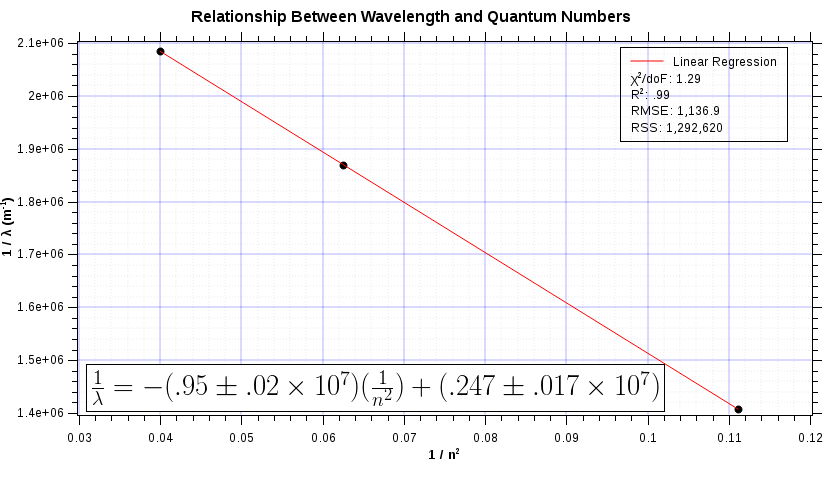
\includegraphics[width=\linewidth]{./Ryberg_graph.png}
	\caption{Plotting the inverse relationships between the wavelength and the corresponding principal quantum number recovers Ryberg's constant as the slope of the linear fit.}
	\label{fig:Ryberg_graph}
	\end{center}
	\par\end{centering}
\end{figure}

Ryberg's Constant, from Graph: \hfill\underline{$.95\pm.02\times 10^7$}

Ryberg's Constant, Theoretical: \hfill\underline{$1.097\times10^7$}

Percent Error: \hfill\underline{13\%}

Bohr radius, experimental, given by
\begin{align*}
	m &= \frac{k_e e^2}{2 a_o h c} \\
	\Rightarrow a_o &= \frac{k_e e^2}{2 m h c}
\end{align*}

\hfill\underline{$a_0 =$ 61.2 $\times 10^{-12}$m}

Bohr Radius, Theoretical: \hfill\underline{$a_{0\text(th)}$ = 52.9 $\times 10^{-12}$m}

Percent Error: \hfill\underline{16\%}

\noindent\hrulefill

\subsection{Part 3: Spectral Emission Lines for H, He, and Hg}
\begin{table}[H]
\centering
\caption{Hydrogen Spectrum}
\begin{tabular}{@{}llccl@{}}
\toprule
\multicolumn{1}{c}{\textbf{Color}} & \multicolumn{1}{c}{\textbf{Intensity}} & \textbf{\begin{tabular}[c]{@{}c@{}}Wavelength(Theory)\\ (nm)\end{tabular}} & \textbf{\begin{tabular}[c]{@{}c@{}}Wavelength(Meas)\\ (nm)\end{tabular}} & \multicolumn{1}{c}{\textbf{\%Error}} \\
\midrule \\
Violet                             & 15                                     & 410.0                                                                      & 417.5                                                                   & 1.9                                  \\
Blue-Violet                        & 30                                     & 434.0                                                                      & 442.9                                                                   & -2.1                                 \\
Blue-Green                         & 80                                     & 486.1                                                                      & 489.7                                                                   & 0.74                                 \\
Red                                & 300                                    & 656.2                                                                      & 649.5                                                                   & -1.0 \\
\bottomrule
\end{tabular}
\end{table}



\begin{table}[H]
\centering
\caption{Helium Spectrum}
\begin{tabular}{@{}llccl@{}}
\toprule
\multicolumn{1}{c}{\textbf{Color}} & \multicolumn{1}{c}{\textbf{Intensity}} & \textbf{\begin{tabular}[c]{@{}c@{}}Wavelength(Theory)\\ (nm)\end{tabular}} & \textbf{\begin{tabular}[c]{@{}c@{}}Wavelength(Meas)\\ (nm)\end{tabular}} & \multicolumn{1}{c}{\textbf{\%Error}} \\
\midrule \\
UV                                 & 500                                    & 388.8                                                                      & 383.7                                                                    & -1.3                                 \\
Blue                               & 200                                    & 447.1                                                                      & 439.6                                                                    & -1.7                                 \\
Green                              & 100                                    & 501.5                                                                      & 509.1                                                                    & 1.5                                  \\
Orange                             & 500                                    & 587.5                                                                      & 579.3                                                                    & -1.4                                 \\
Red                                & 100                                    & 667.8                                                                      & 661.2                                                                    & -0.99                                \\
IR                                 & 200                                    & 706.5                                                                      & 697.9                                                                    & -1.2                                \\
\bottomrule
\end{tabular}
\end{table}


\begin{table}[h]
\centering
\caption{Mercury Spectrum}
\begin{tabular}{@{}llccl@{}}
\toprule
\multicolumn{1}{c}{\textbf{Color}}                       & \multicolumn{1}{c}{\textbf{Intensity}} & \textbf{\begin{tabular}[c]{@{}c@{}}Wavelength(Theory)\\ (nm)\end{tabular}} & \textbf{\begin{tabular}[c]{@{}c@{}}Wavelength(Meas)\\ (nm)\end{tabular}} & \multicolumn{1}{c}{\textbf{\%Error}} \\ \midrule
UV                                                       & 2800                                   & 365                                                                        & 369.6                                                                    & 1.26                                 \\[8pt]
Violet                                                   & 1800                                   & 404.6                                                                      & 405.99                                                                   & 0.34                                 \\[8pt]
\begin{tabular}[c]{@{}l@{}}Blue-\\ Violet\end{tabular}   & 4000                                   & 435.8                                                                      & 435.2                                                                    & -0.14                                \\[8pt]
\begin{tabular}[c]{@{}l@{}}Blue -\\ Green\end{tabular}   & 90                                     & 491.6                                                                      & NA                                                                       & NA                                   \\[8pt]
Yellow                                                   & 1100                                   & 546                                                                        & 541.92                                                                   & -0.75                                \\[8pt]
\begin{tabular}[c]{@{}l@{}}Yellow-\\ Orange\end{tabular} & 280                                    & 579                                                                        & 572.08                                                                   & -1.20                                \\[8pt]
\begin{tabular}[c]{@{}l@{}}Orange-\\ Red\end{tabular}    & 1000                                   & 614.9                                                                      & 691.18                                                                   & 12.41                                \\ \bottomrule
\end{tabular}
\end{table}

%\bibliographystyle{plain}
%\bibliography{physbib}

\end{document}